\documentclass[a4paper, 11pt]{article}
\setlength{\topmargin}{0.0in}
\setlength{\textheight}{9.5in}
\setlength{\oddsidemargin}{-.1in}
\setlength{\textwidth}{6.5in}
\usepackage{parskip}
\usepackage{graphicx}
\graphicspath{ {images/} }
\usepackage{datetime}

\newdateformat{monthyeardate}{%
  \monthname[\THEMONTH], \THEYEAR}

\date{}
\begin{document} 

\LARGE\title{Real Time Tempo Analysis of Drum Beats}

\LARGE\author{Author: \textbf{Philip Hannant}, Supervisor: \textbf{Professor Steve Maybank}\\
\\Birkbeck, University of London\\
Department of Computer Science and Information Systems\\
\\Project Report\\
MSc Computer Science\\
\\\monthyeardate\today
}





\normalsize


\maketitle
\newpage
\tableofcontents
\clearpage

\section*{Abbreviations}
\begin{tabular}{l p{4.5in}  }\\
\textbf{BPM} & Beats Per Minute\\
\textbf{DWT} & Discrete Wavelet Transform\\
\textbf{FFT} & Fast Fourier Transform\\
\textbf{JSON} & Javacript Object Notification\\
\textbf{IDE} & Integrated Development Environment\\
\textbf{TDD} & Test Driven Development\\
\end{tabular}

\section*{Definitions}
\begin{tabular}{l p{4.5in}}\\
\textbf{Acoustic Drum Kit} & A collection of drums and cymbals which do not have electronic amplification. Typically made up of a bass drum, snare drum, tom-toms, hi-hat and 1 or more cymbals.\\\\
\textbf{Beat} & For the purpose of this project a beat will be defined as the sequence of equally spaced pulses used to calculate the tempo being played by the drummer.\\\\
\textbf{Downbeat} & Refers to beat one of a measure of music, called a downbeat to correspond to the motion a conductor's arm [1].\\\\
\textbf{Drum Module} & The device which serves as a central processing unit for an electronic drum kit, responsible for producing the sounds of the drum kit.\\\\
\textbf{Electronic Drum Kit} & An electrical device which is played like an acoustic drum kit, producing sounds from a stored library of instruments and samples.\\\\
\textbf{MIDI} & Musical Instrument Digital Interface is a protocol developed in the 1980's to allow electronic instruments and other digital musical tools to communicate with each other [3].\\\\
\textbf{Tempo} & The speed at which a piece of music is played \cite{oxford-comp} and counted in beats per minute (bpm).\\\\
\end{tabular}
\clearpage

\maketitle{} \section{Introduction and Background}

This project report presents my aim to develop a real-time drum beat tempo analysis system using different beat detection algorithms which is able to record the perfomance of each method concurrently when an extensive set of drum samples, representing a real drummer's perfomance, is processed through the system.

\subsection{Drumming Training Tools Background}
Timing is the fundamental skill any good drummer should possess and is the staple by which they will be judged. For many years the only training tool available to a drummer to improve their timing was the metronome. An instrument used to mark musical tempo, erroenously attributed to Johann Nepomuk Maelzel in 1815 but was actually invented by a Dutchman, Dietrich Nikolaus Winkel a year earlier. The traditional metronome, based on Winkel's original design is a hand-wound clockwork instrument that uses a pendulum swung on a pivot to generate the ticking which depicts the desired tempo \cite{brit-metro} is still used today by musicians, as seen in Figure~\ref{fig: TradMet}. \par

\begin{figure}[ht]
	\centering
	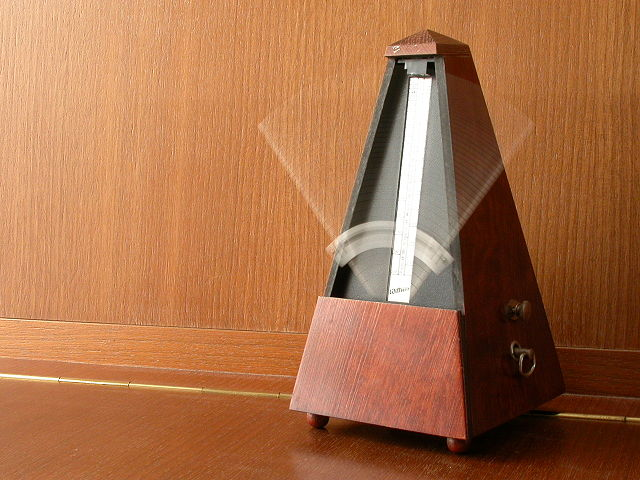
\includegraphics[scale=0.30]{TradMet}
	\caption{Traditional Metronome}% (Source: https://commons.wikimedia.org/w/index.php?curid=1058005)}
	\label{fig: TradMet}
\end{figure}

For drummers however the electronic versions of the metronome are much more widely used, to the point that metronomes are now developed with functionality specifically tailored to a drummers training requirements. The Tama Rhytham Watch (Figure~\ref{fig: RW200}) was the first metronome designed specifically for drummers, providing enough volume to be used with real drums as well as allowing for the use of different time signatures and preset set rhythm patterns to help improve perfomance.\par
\clearpage

\begin{figure}[ht]
	\centering
	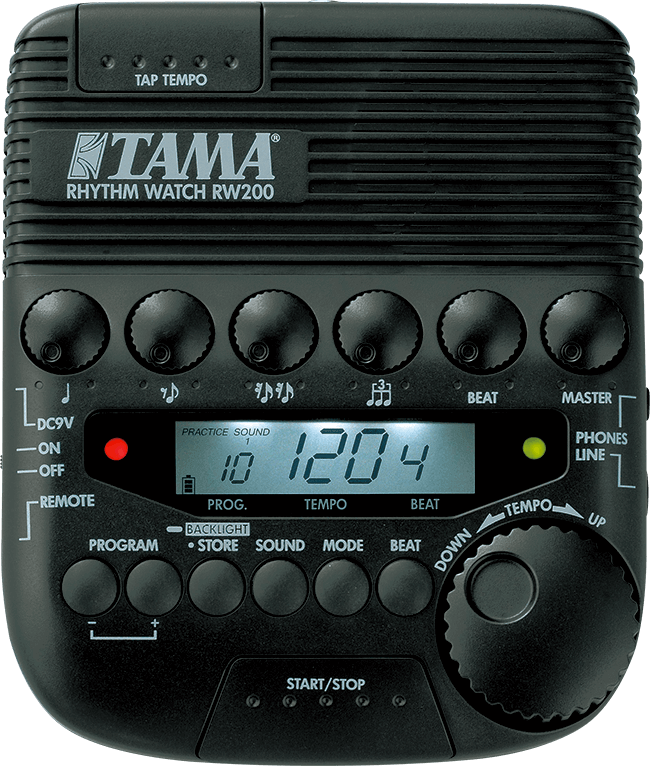
\includegraphics[scale=0.25]{RW200}
	\caption{Tama Rhythm Watch}% (Source: http://www.tama.com/eu/products/accessories/RW200.html)}
	\label{fig: RW200}
\end{figure}

Following the development of MIDI driven electronic drum kit came the development of more advanced training tools that now were able to provide live feedback to drummer during any given perfomance. Today the leaders in this field are Roland, their v-drums line provide a variety of tutition packages including the SCOPE and more recently the COACH system provided in the v-drum modules, the v-drum Rhymthm Coach line is an advanced version of the traditional drummers practice pad and the extensive DT-1 V-Drums tutor software package. Roland have even now gamified this field with their latest release, the V-Drums Friend Jam app. The application itself provides the player with live feedback and evaluates each performance in order to provide the player with a score which they can share over social media. \par

The aim of this project is to investigate whether some of the current beat detection algorithms available would be accurate enough to provide the basis for a training tool for dummers using an acoustic drum kit as opposed to an electronic drum kit. \par

\subsection{Drum Musical Theory}
In order to understand the fundamentals of musical timing some theory needs to be examined but beforehand the concept of a drummer playing time must be considered. Time, in a drumming sense is an informal term used to describe the consistent rhythmic pattern that a drummer will play on the hi-hat or ride cymbal \cite{drum-bible} and it can be considered one of the most important components of any drum beat. 

\subsubsection{Notation}
Drum music notation is written on staff that is made up of five individual lines, the clef is found on the far left of the staff which indicates the pitch of the notes \cite{oxford-comp} and as percussion instruments are non-pitched they use the percussion-clef. On traditional musical notation the lines and spaces between represent a tonal where as for drum notation, notes written on lines or spaces indicate a certain drum or cymbal. The staff is seperated into individual measures which are known as bars \cite{drum-note} and it is these bars that are the basis of musical time. For the purpose of this project it is the count of these beats that will be used to calculate the tempo of a certain drum beat.

\subsubsection{Time Signatures}
Time signatures appear on the staff just after the clef and are written as a fraction where the top number indicates the number of beats that there are in a bar. With the bottom number representing the size of the note that makes up the duration of one beat. For example the straight time four four (4/4) or common time signature indicates four beats in each bar or measure where each beat is made up of one quarter note \cite{drum-note}. Within these bar lines beats can be further divided by using a technique known as subdivision, which is a method for reducing the pulse or rhythm pattern into smaller parts than those originally written, for example counting a four four (4/4) measure in eighth (1/8) or sixteeth (1/16) notes. 

\subsubsection{Notes}
The notes used to represent the percussive instrument to be played also provide the duration it should be played for. Notes come in different lengths and the key values are the whole (1/1), half (1/2), quarter (1/4), eighth (1/8) and sixteeth (1/16). For example two eighth notes represent the same time value as a single quarter note. It is possible to divide a note values by three instead of two, these notes are known as triplets. An eighth note triplet is played fifty percent faster than a normal eighth note, therefore for every two eighth notes there will be three eighth note triplets \cite{drum-note}. An example of the eighth-note triplets being used is in a twelve eight (12/8) jazz shuffle, the time element played on the ride cymbal or hi-hat is charaterised by playing the first and third triplet of an eighth-note triplet grouping \cite{drum-bible}.

\subsubsection{Playing Basics}
With the basics of drum theory covered it is now possible to discuss the key elements of a drum beat, typically for a straight four four (4/4) bar the bass drum will be played on the first and third beat and the snare drum will be played on the second and forth beat both as quarter notes. This is more commonly known as a back beat \cite{drum-bible}. This just leaves the time element which will usually be played on the ride cymbal or hi-hat, this too could be played using quarter notes on the first, second, third and forth beats. However, in order to make the drum pattern more dynamic the time element will usually be played using subdivisions, typically using eighth note subdivisions. The ride cymbal or hi-hat will therefore be played on the first, second, third and forth beats as well as the eighth notes inbetween each quarter note. This can be demostrasted by counting the one-and-two-and-three-and-four-and, where the and represents the subdivided eighth note. Additonally to this technique a drummer will usually ensure that there is difference in the volume of the eighth notes being played on the quarter notes and those being played on the and. This technique of emphasising certain beats is known as accenting. 


\subsection{Beat Detection Background}
Most of the early work on beat detection was a by-product of research directed at other areas of musicical understanding. The earliest work in this field can be attributed to H. C. Longuet-Higgins, who in 1976 while researching the psychological theory of how Western musicians perceive rhythmic and tonal relationships between notes. Produced an algorithm that was able to follow the beat of a performance and adjust the perceived tempo accordingly based on whether a note started earlier or later than expected \cite{allen-danneburg}. Longuet-Higgins' work was built on the premise that in order to percieve the rhythmic structure of a melody it is first necessary to identify the time at which each beat occurs \cite{longeut1}, otherwise know as onset detection. The onset of a note is the instant which marks start of the variation in the frequency of a signal, a visualisation of this can be seen in Figure~\ref{fig: Onset}. Once detected it can then be used to measure the onset times of sonic events\footnote{A sonic event is a singular feature of a piece music which can be made up of one source or many\cite{sonic}, e.g. the hitting of a drum} within a piece of music\cite{mirex-onset}. These onset times are then used within a beat detection algorithm in order to calculate the piece of music's tempo. 

\begin{figure}[h]
	\centering
	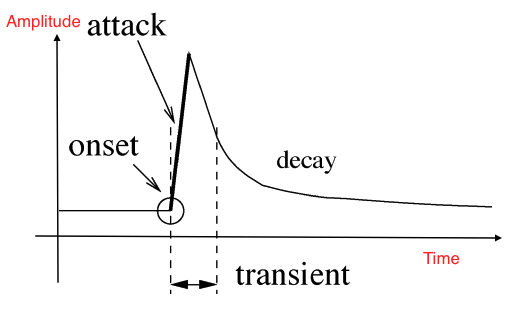
\includegraphics[scale=0.40]{Onset}
	\caption{The onset of a note is the instant which marks start of the variation in the frequency of a signal (Image Source: \cite{onset-tut})}
	\label{fig: Onset}
\end{figure}

Since Longuet-Higgins' first work the are of beat detection has expanded rapidly, in 2005 the first annual Music Information Retrieval Evaluation eXchange (MIREX) was held in 2005. MIREX includes a contest with the goal of comparing state-of-the-art algorithms for music information retrieval \cite{mirex-main}. The topics to be evaluated are proposed by the participants. In the first year, three of the nine topics concerned beat detection, including audio onset detection and since it's first inclusion it has been an evalulated topic of all but one of the last twelve contests \cite{mirex-onset}. The beat detection algorithms proposed to perform the tempo analysis for this project, the Beatroot system developed by Simon Dixon \cite{dixon1} and a development on the original audio analysis using the Discrete Wavelet Transform (DWT) by Tzanetakis, Essel and Cook \cite{tzane1}. Are both former entrants the MIREX contest, with the beatroot system receiving the highest score in the 2006 Audio Beat Tracking task \cite{mirex-06} 

\subsection{Project Aims}
The primary aim of this project is to investigation whether some of the currently avaliable beat detection algorthims are accurate enough to form the basis for a training tool to be used by drummers practicing on an acoustic drum kit. In order to achieve this the developed software package, hereafter referred to as  RTT\_Analyser\footnote{Where RTT stands for Real Time Tempo}, will need to process enough live audio in form of preconstructed drum beats and record each of the chosen beat detection algorithms accuracy. 

The original core features of the RTT\_Analyser developed for this project are:

\begin{enumerate}
\item A live audio tempo analysis tool, that compares and records the performance of selected beat detection algorithms
\item The RTT\_Analyser implements an adapted version of the beat tracking system Beatroot and Discrete Wavelet Transform algorithm described by Tzanetakis \textit{et al}'s\cite{tzane1} which process live audio as opposed to originally designed off-line audio files.
\item RTT\_Analyser implements a concurrent system that provides the same captured live audio data to the chosen beat detection algorithms in order for the tempo to be calculated simultaneously.
\item While processing live audio the RTT\_Analyser stores a predetermined data set in order to allow for performance analysis of the beat detection algorithms.
\item The RTT\_Analyser will provide the user with real time feedback of the most recent tempo calculation returned
\item In order to An extensive sample set of drum beats will need to be created to ensure the system is tested sufficiently
\end{enumerate}

\maketitle{} \section{Solution Design}
add something about work flow of system plus detailed work flow diagram

\subsection{RTT\underline{{ }}Analyser Beat Detection}
The original proposed solution incorporated two beat detection logarithms, Beatroot system \cite{dixon1} and the DWT method \cite{tzane1}. However during the development the adaptation of the Beatroot system to be used with live audio took longer than the proposed time-frame. This meant that an alternative system needed to be found in order to mitigate this issue, conveniently the Beatroot software package also contained another beat detection system, the Performance Worm \cite{dixon3}. In order to ensure the project remained on track it was decided to substitute the Performance Worm for the Beatroot system. The intention was, if time allowed, to resume the adaptation of the Beatroot system to work with live audio once the project was ahead of schedule and this was successfully completed prior to the development of the user interface.

The project report will now discuss all of the beat detection alogrithms that were incorporated in the RTT\_Analyser as well as the system used to allow for simultaneous tempo calculation.  

\subsubsection{Beatroot}
Beatroot is a beat detection software package created by Simon Dixon \cite{dixon1}, which was orignally designed extract musical expression information musical recordings\cite{dixon3}. Beatroot was included in the RTT{\_}Analyser as the algortihm designed by Dixon was considered to be sufficiently fast enough to be implemented as part of a real-time system\cite{dixon4}.\par

Beatroot works by first obtaining a time-frequency representation of the signal based on a Short Time Fourier Transform (STFT) using a Hamming window\cite{dixon2}. The STFT is a form of Fourier transform (FT), which can be used to find out how much of each frequency exists in a signal. Th A negative of the FT is that it is unable to provide any details of when a frequency component occurs in time for non-stationary signals\footnote{Non-stationary signals are signals whose frequency contents changes over time\cite{polikapt2}}. A solution to this is to split a non-stationary signal up into a number of smaller segments using a window function, which effectively created a series of stationary\footnote{The frequency contents of a stationary signal does not change over time} signals which the FT could then be applied to. The STFT will then be able to blah blah. The Hamming window function is used to reduce leakage and is characterised by the reducing amplitudes of its sidelobes and the appearence that it is raised on a \textit{pedestal}\cite{lyons}. A visualisation of a Hamming window can be seen in Figure~\ref{fig: hamWin}. 

\begin{figure}[h]
	\centering
	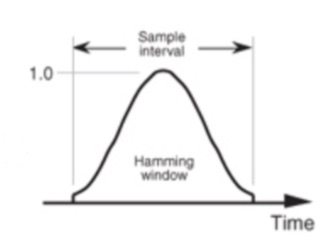
\includegraphics[scale=0.36]{hamWin}
	\caption{(Image Source: \cite{lyons})}
	\label{fig: hamWin}
\end{figure}

Once the time-frequency representation is returned the next stage is to the spectral flux onset detection function, which is a method for measuring the change in magnitude of each returned frequency bin\cite{dixon2}. The onsets are then selected from the spectral flux onset detection function by a peak-picking algorithm which finds local maxima within the dectection function. The next stage is to apply the tempo induction algorithm which is used to compute clusters of inter-onset intervals (IOI) by using the calculated onset times. Each cluster represents a hypothetical tempo, in seconds per beat \cite{dixon1}. The clustering algorithm works by assigning an IOI to a cluster if its difference from the cluster is less than 25ms. The cluster information is then combined by recognising the approximate integer relationships between clusters. An example of this can be seen in Figure~\ref{fig: br-clusters} where cluster C2 is twice as long as C1 and C4 is twice that of C2. This information along with the number of IOIs within a cluster is then used to weight each cluster which is then returned as a ranked list of tempo hypotheses\cite{dixon4}.

\begin{figure}[h]
	\centering
	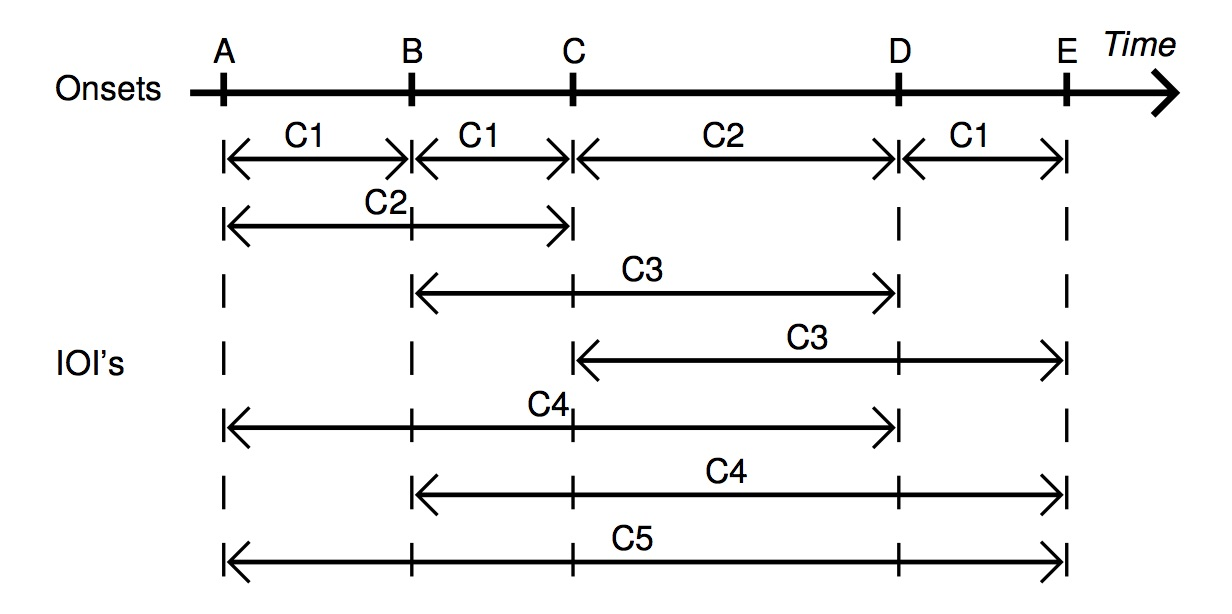
\includegraphics[scale=0.25]{br-clusters}
	\caption{(Image Source: \cite{dixon4})}
	\label{fig: br-clusters}
\end{figure}

The multiple agent architecture of Beatroot's beat tracking subsystem is then employed to find the sequences of events that closest match the original tempo hypotheses, each of these sequences is then rated and the most likely set of beat times is determined.


\subsubsection{Discrete Wavelet Transform}
The first literature regarding the wavelet was provided by the mathematician Albert Haar in 1909 [18]. The wavelet transform is a technique for analysing signals which was developed as an alternative to the STFT [11]. Like the STFT, the DWT is able to provide time and frequency information, however, unlike the STFT the DWT is able to do this without the need for a window function. 

\subsubsection{Tzanetakis \textit{et al} Beat Detection Method}
In 2001, Tzanetakis \textit{et al} described how the Discrete Wavelet Transform (DWT) could be used to extract information from non-speech audio [11]. Their beat detection algorithm was based on detecting the most prominent signals which are repeated over a period of time within the analysed audio and was is split into the following stages: 

\begin{itemize}
\item DWT - First the signal is processed by the DWT into a number of frequency bands 
\item Low Pass Filtering - a low pass filter is then applied to the signal in order to allow the lower frequencies of the signal to be analysed
\item Full Wave Rectification - each frequency band is then converted to one constant polarity (positive or negative)[wiki]. A visual representation can be seen in Figure 4
\item Downsampling - the sampling rate of the signal is decreased by an integer factor [20]
\item Normalisation - each band is then normalised using mean removal
\item AutoCorrelation - an autocorrelation function is then applied to the frequency bands, the first five peaks of this function are detected and their periodicities are calculated in beats per minute
\end{itemize}





\maketitle{} \section{Implementation}
\subsection{Live Audio Processing}
The live audio will be processed using the Javax Sound package. The audio will be captured using a stereo microphone and processed to match CD quality with the Javax Sound AudioFormat class. The Beatroot system was not originally intended to be used as a real time system [19] so currently only works with prerecorded audio. It will therefore be will need to be modified in order for it to work with live audio. 

\begin{itemize}
\item Encoding - This will be set to ``PCM.signed'', representing audio encoded to the native linear pulse code modulation, where quantization levels are linearly uniform [15].
\item Sample Rate - 44,100, set to match CD quality for the number of analog samples which will be analysed per second. 
\item Sample Size in Bits - 24, based on a sound card with a 24 bit sample depth.
\item Channels - 2, audio will be captured using a stereo microphone.
\item Frame Size - 6, where the frame size is the number of bytes in a sample multiplied by the number of channels [17].
\item Frame Rate - 44,100, same as sample rate.
\item Big Endian (boolean) - false, as the project will be developed on an Intel core which uses a little-endian architecture\footnote{Endianess refers to the order of bytes which make up a digital word. Big endianess stores the most significant byte at a certain memory address and the remaining bytes being stored in the following higher memory addresses. The little-endian formate reverses the order storing the least significant at the lowest and most significant at the highest memory address [16].}.
\end{itemize}


\newpage
\begin{thebibliography}{99}
\bibitem{brit-metro} 
\textit{https://www.britannica.com/art/metronome}
\bibitem{drum-bible}
Mick Berry and Jason Gianni
\textit{The Drummer's Bible: How to Play Every Drum Style from Afro-Cuban to Zydeco, Second Edition, 2004, See Sharp Press}
\bibitem{oxford-comp}
Alison Latham
\textit{The Oxford Companion to Music, 2002, Oxford University Press}
\bibitem{drum-note}
\textit{http://www.drummagazine.com/lessons/post/drumkey/}
\bibitem{allen-danneburg}
Allen and Dannenberg
\textit{Tracking Musical Beats in Real Time, International Computer Music Conference, International Computer Music Association, 1990, pp. 140-143}
\bibitem{longeut1}
H. C Longuet-Higgins
\textit{Perception of melodies, Nature Vol. 263, 1976, pp. 646-653}
\bibitem{dixon1}
Simon Dixon
\textit{Automatic Extraction of Tempo and Beat from Expressive Performances. Journal of New Music Research, 30 (1), 2001, pp 39-58}
\bibitem{dixon2}
Simon Dixon
\textit{Onset Detection Revisited, Proceedings of the 9th International Conference on Digital Audio Effects, Montreal, September 2006, pp 133-137}
\bibitem{dixon3}
Simon Dixon
\textit{On the Analysis of Musical Expression in Audio Signals. Storage and Retrieval for Media Databases, SPIE-IS\&T Electronic Imaging, SPIE Vol. 5021, 2003 pp 122-132}
\bibitem{mirex-onset}
\textit{http://www.music-ir.org/mirex/wiki/2016:Audio\_Onset\_Detection}
\bibitem{sonic}
\textit{http://www.ieor.berkeley.edu/~ieor170/sp15/files/Intro-to\_Sonic\_Events\_Campion.pdf}
\bibitem{onset-tut}
Juan Pablo Bello, Laurent Daudet, Samer Abdallah, Chris Duxbury, Mike Davies, and Mark B. Sandler 
\textit{A Tutorial on Onset Detection in Music Signals, IEEE TRANSACTIONS ON SPEECH AND AUDIO PROCESSING, VOL. 13, NO. 5, 2005, pp. 1035 - 1047}
\bibitem{mirex-main}
\textit{http://www.music-ir.org/mirex/wiki/2005:Main\_Page}
\bibitem{tzane1}
George Tzanetakis, Georg Essl and Perry Cook
\textit{Audio Analysis using the Discrete Wavelet Transform, Proc. WSES International Conference on Acoustics and Music: Theory and Applications (AMTA), 2001}
\bibitem{mirex-06}
\textit{http://www.music-ir.org/mirex/wiki/2006:Audio\_Beat\_Tracking\_Results}
\bibitem{dixon4}
Simon Dixon
\textit{Evaluation of the Audio Beat Tracking System BeatRoot. Journal of New Music Research, 36, 1, 2007, pp 39-50}
\bibitem{polikapt2}
\textit{http://users.rowan.edu/ polikar/WAVELETS/WTpart2.html}
\bibitem{lyons}
Lyons
\textit{Understanding Digital Signal Processing}
\end{thebibliography}
\end{document}

